% 2026-10-23：按学习复现、探索尝试、优化验证、迭代调试、整板尝试重组。
\documentclass[stage2,fontset=fandol]{ydzjreport}
\usepackage{subcaption,longtable}

\stagetwosetup
{第 2 个逻辑月 · 探索与尝试}
{冯旭东、陈思文、张昊洋}
{复合微通道分区冷却}
{【待确认】逻辑月 2 对应的自然月}
{多种小块；代表结构比较；传统 PID；控制流程}
{探索不同小块结构的温度与水力表现，形成翼型专题研究的动机；学习传统 PID 的具体知识并提出控制流程。}
\pagestyle{empty}   % 去掉页眉与页脚（含页码）
\RemoveFromHook{enddocument}[ydzjreport] % 去掉末页的作者与格式规范收尾说明


\newlabel{sub@fig:zhixian-t}{{a}{6}{直线流道温度\relax }{figure.caption.7}{}}
\newlabel{sub@fig:zhixian-p}{{b}{6}{直线流道静压\relax }{figure.caption.7}{}}
\newlabel{sub@fig:zhixian-v}{{c}{6}{直线流道速度大小\relax }{figure.caption.7}{}}
\newlabel{sub@fig:zhixian-cu}{{d}{6}{直线流道铜板温度\relax }{figure.caption.7}{}}
\newlabel{sub@fig:sin-t}{{e}{6}{正弦流道温度\relax }{figure.caption.7}{}}
\newlabel{sub@fig:sin-p}{{f}{6}{正弦流道静压\relax }{figure.caption.7}{}}
\newlabel{sub@fig:sin-v}{{g}{6}{正弦流道速度大小\relax }{figure.caption.7}{}}
\newlabel{sub@fig:sin-cu}{{h}{6}{正弦流道铜板温度\relax }{figure.caption.7}{}}
\newlabel{sub@fig:naca-t}{{i}{6}{NACA2416 温度\relax }{figure.caption.7}{}}
\newlabel{sub@fig:naca-p}{{j}{6}{NACA2416 静压\relax }{figure.caption.7}{}}
\newlabel{sub@fig:naca-v}{{k}{6}{NACA2416 速度大小\relax }{figure.caption.7}{}}
\newlabel{sub@fig:naca-cu}{{l}{6}{NACA2416 铜板温度\relax }{figure.caption.7}{}}
\newlabel{sub@fig:gao-t}{{m}{6}{gao2.1 温度\relax }{figure.caption.7}{}}
\newlabel{sub@fig:gao-p}{{n}{6}{gao2.1 静压\relax }{figure.caption.7}{}}
\newlabel{sub@fig:gao-v}{{o}{6}{gao2.1 速度大小\relax }{figure.caption.7}{}}
\newlabel{sub@fig:gao-cu}{{p}{6}{gao2.1 铜板温度\relax }{figure.caption.7}{}}
\begin{document}
\section*{逻辑月2\_指标与形态：图表附件}
本附件图表编号与对应提交正文及完整报告一致。\par\clearpage
\setcounter{table}{0}
\begin{table}[H]
\centering
\caption{本阶段文献与资料}
\label{tab:lit}
\begin{tabularx}{\textwidth}{@{}c Y Y@{}}
\toprule
\rowcolor{ydzjlight} 序号 & 文献与资料 & 解决了我哪个问题 \\
\midrule
1 & 四种流道数据与折线图 & 确定有效工况与比较条件 \\
2 & NACA 翼型数据 & 识别可用于后续分组的厚度、弯度与攻角参数 \\
3 & 复合叶脉蜂窝微通道等仿生拓扑研究 & 提供仿生结构的设计参照 \\
4 & 控制理论教材与 PID 专著\cite{hushousong,astrom,franklin,ogata} & 确定控制回路结构、基础控制器形式与整定思路 \\
\bottomrule
\end{tabularx}
\end{table}
\clearpage
\setcounter{table}{1}
\begin{table}[H]
		\centering
		\caption{PID 三个作用的物理含义与代价}
		\label{tab:pid}
		\begin{tabularx}{\textwidth}{@{}c Y Y Y@{}}
			\toprule
\rowcolor{ydzjlight} 作用 & 物理含义 & 带来什么 & 代价 \\
			\midrule
			P & 与当前误差成正比 & 立即响应，提高增益可加快响应 & 留下稳态误差；增益过大会振荡 \\
			I & 累积历史误差 & 消除稳态误差（提高无差度） & 引入约 $-90^\circ$ 相位滞后，易超调；长时间饱和会积分饱和 \\
			D & 对误差变化率作用 & 提供超前相位，改善阻尼、抑制超调 & 放大测量噪声；对纯滞后补偿能力有限 \\
			\bottomrule
		\end{tabularx}
	\end{table}
\clearpage
\setcounter{table}{2}
\begin{table}[H]
		\centering
		\caption{物理性质与控制设计的对应关系}
		\label{tab:physics-control}
		\begin{tabularx}{\textwidth}{@{}Y Y@{}}
			\toprule
\rowcolor{ydzjlight} 对象性质 & 对控制设计的含义 \\
			\midrule
			一阶惯性（时间常数 $\tau$） & 需要积分作用消除稳态误差；增益过高会引起振荡 \\
			纯滞后（FOPDT） & 可考虑超前或预测方法，需检验时延影响；滞后越大，可用增益越低 \\
			执行器饱和（泵 $0$--$6000$ RPM、阀 $0$--$100\%$） & 必须做抗积分饱和，否则长时间饱和后积分项会积累成大幅超调 \\
			换热系数收益递减（$n<1$） & 存在「经济流量区间」，超出后加大流量只增加泵功 \\
			临界约束（结温上限） & 需要独立的安全约束层，优先于性能目标 \\
			\bottomrule
		\end{tabularx}
	\end{table}
\clearpage
\setcounter{figure}{0}
\begin{figure}[H]
		\centering
		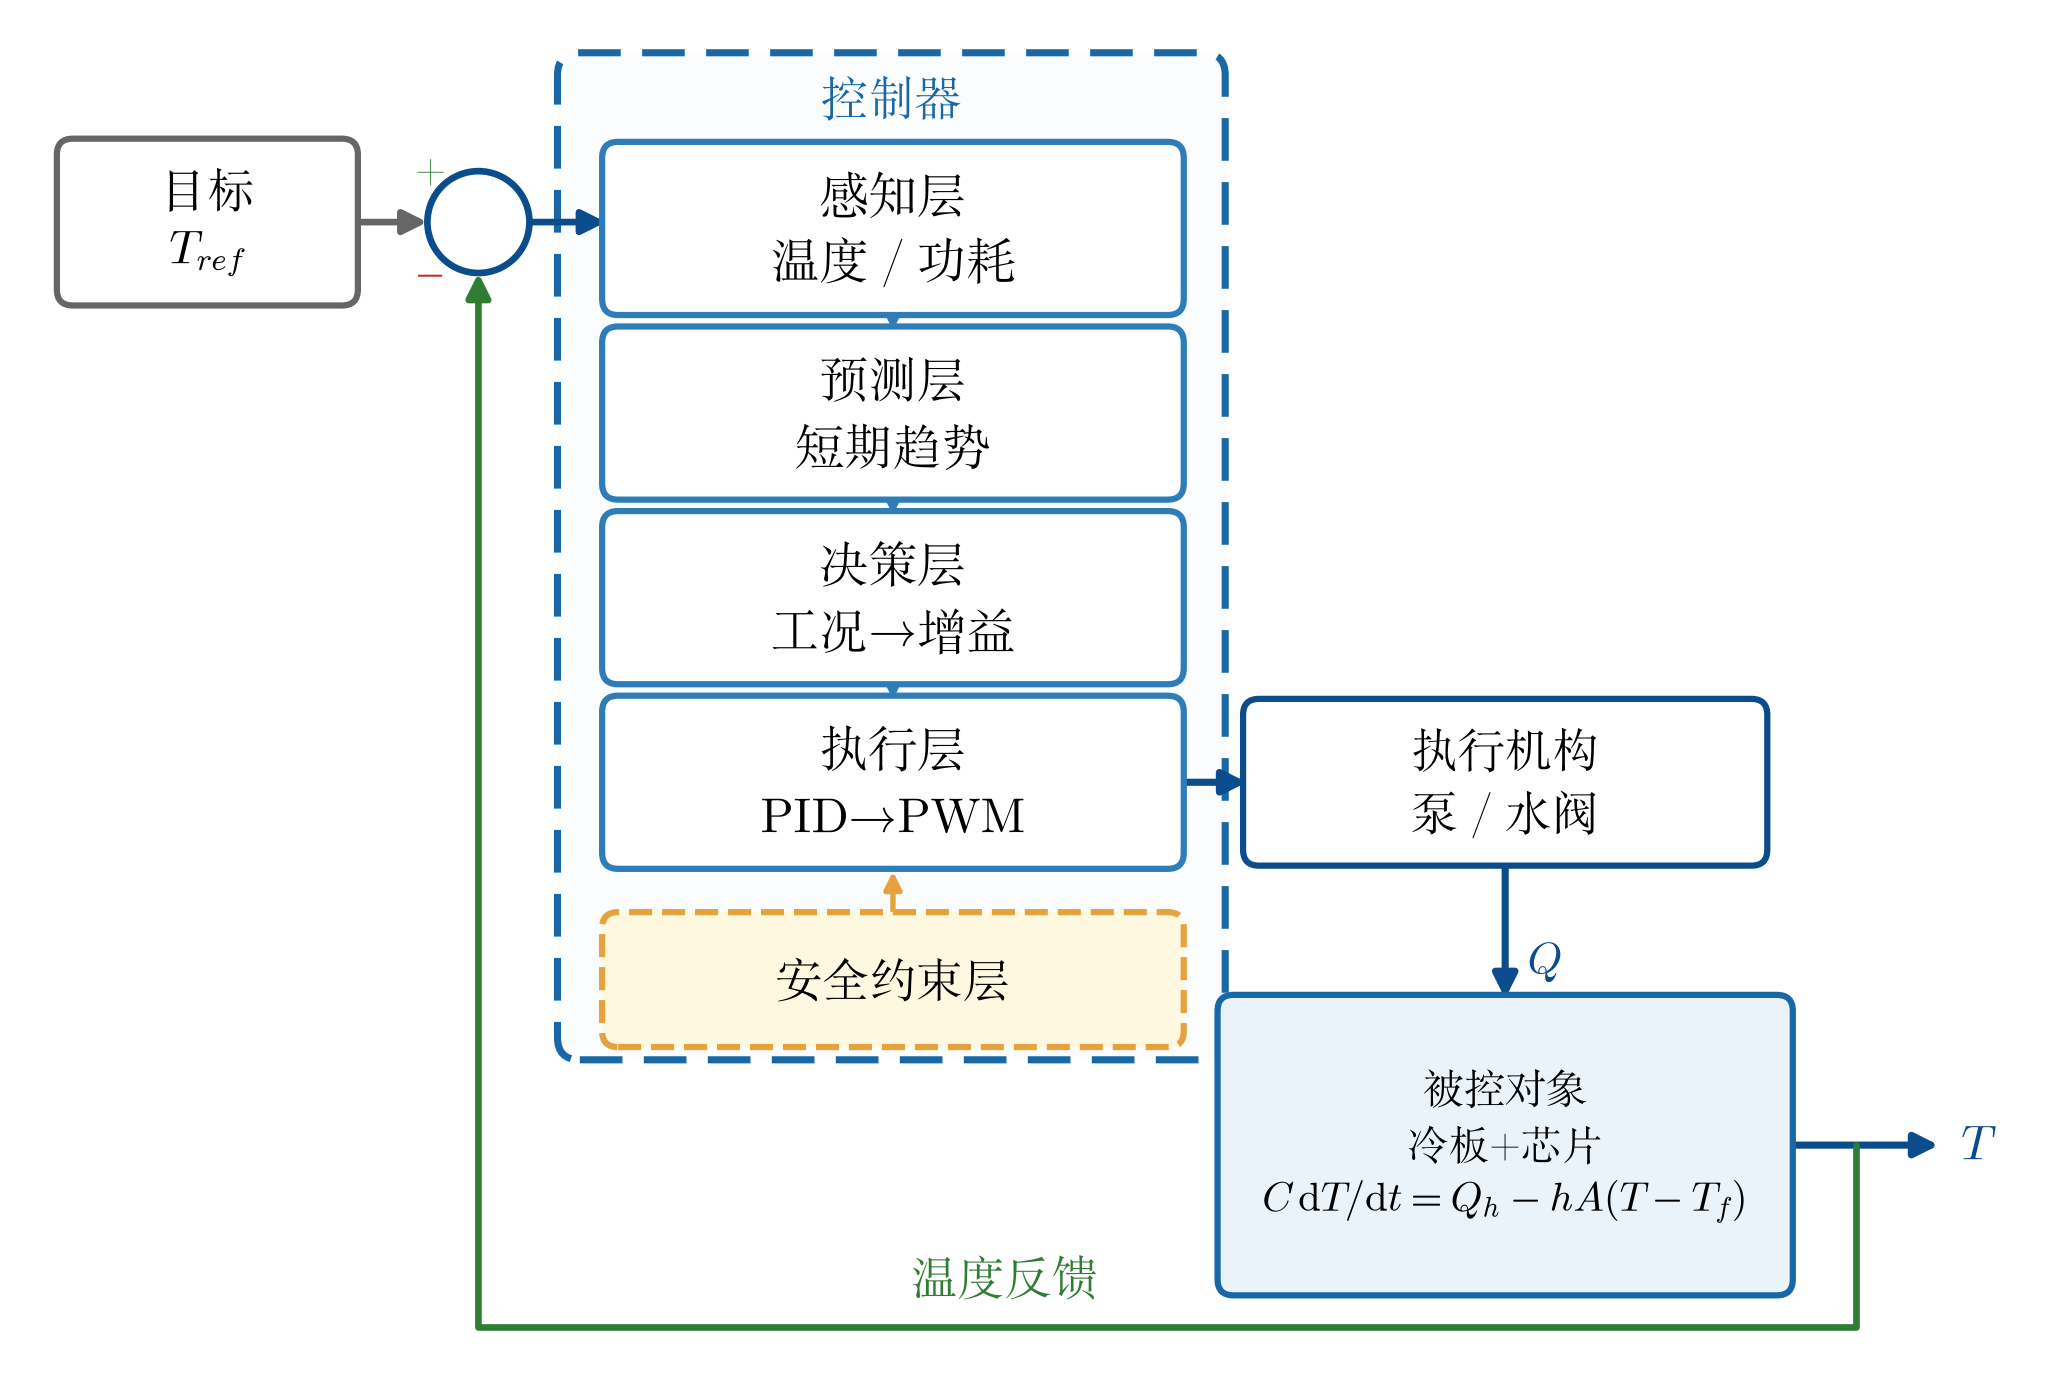
\includegraphics[width=0.97\textwidth]{../../figs/13_控制框架框图.png}
		\caption{动态调控初步框架：感知—预测—决策—执行四层，外挂独立的安全约束层}
		\label{fig:ctrl-framework}
	\end{figure}
\clearpage
\setcounter{table}{3}
\begin{table}[H]
		\centering
		\caption{分层递阶控制器的职责划分与本阶段状态}
		\label{tab:layers}
		\begin{tabularx}{\textwidth}{@{}>{\RaggedRight\arraybackslash}p{0.13\textwidth} Y Y Y@{}}
			\toprule
\rowcolor{ydzjlight} 层 & 输入 & 输出 & 本阶段状态 \\
			\midrule
			感知层 & 传感器测点温度、功耗 & 温度 $T$、变化率 $\mathrm{d}T/\mathrm{d}t$ & 方案已定，测点布置待定 \\
			预测层 & 温度／功耗历史数据 & 短期温度或热流趋势 & \textbf{待建立}（需先积累数据） \\
			决策层 & 趋势 + 当前工况 & PID 增益组合 & 框架已定，整定待做 \\
			执行层 & 误差 $e$ + 当前增益 & PWM 占空比 & PID 结构已定 \\
			安全约束层 & 温度、执行器状态 & 限幅、积分冻结 & 约束原则已提出，阈值待定 \\
			\bottomrule
		\end{tabularx}
	\end{table}
\clearpage
\setcounter{table}{4}
\begin{table}[H]\centering
\caption{本月工作与材料状态}\label{tab:tasks}
\begin{tabularx}{\textwidth}{@{}Y Y Y@{}}
\toprule
\rowcolor{ydzjlight} 工作 & 状态 & 依据或缺口 \\
\midrule
多种结构探索 & 已有结果 & 五条流道代表记录、十七条小模型分支及六翼型基准结果 \\
评价口径 & 部分统一 & 热负荷、流量、时刻及温度统计仍需分别标识 \\
翼型专题方向 & 提出 & 本月合并展示已有结果，参数分组与机理研究后续进一步探究 \\
传统 PID 与控制流程 & 已整理 & 具体知识、控制层次和接口；本月不报告闭环模拟结果 \\
\bottomrule\end{tabularx}\end{table}
\clearpage
\setcounter{figure}{1}
\begin{figure}[H]
\centering
% month2-unified-figure
\resizebox*{!}{0.82\textheight}{%
\begin{minipage}{\textwidth}
\centering
	\begin{subfigure}{0.235\textwidth}
		\centering
		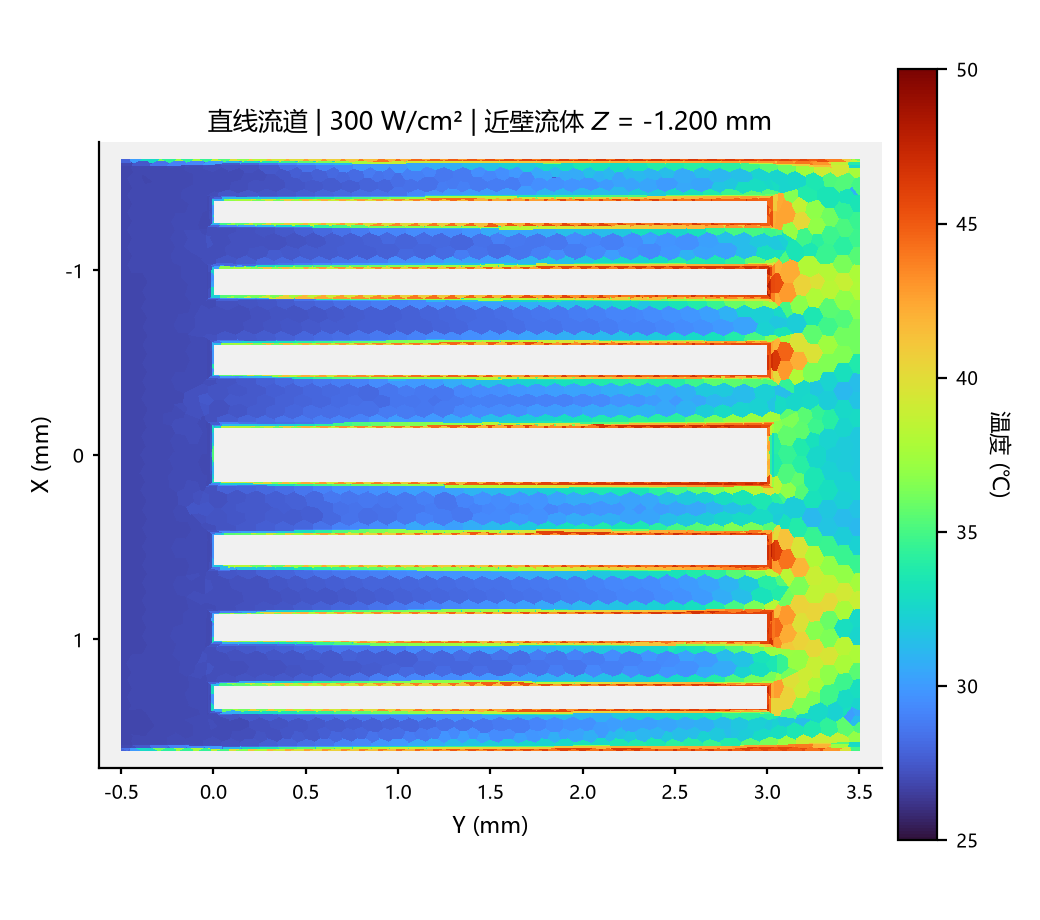
\includegraphics[width=\linewidth]{../../figs/14_zhixian_temperature.png}
		\caption{直线流道温度}
		\label{fig:zhixian-t}
	\end{subfigure}\hfill
	\begin{subfigure}{0.235\textwidth}
		\centering
		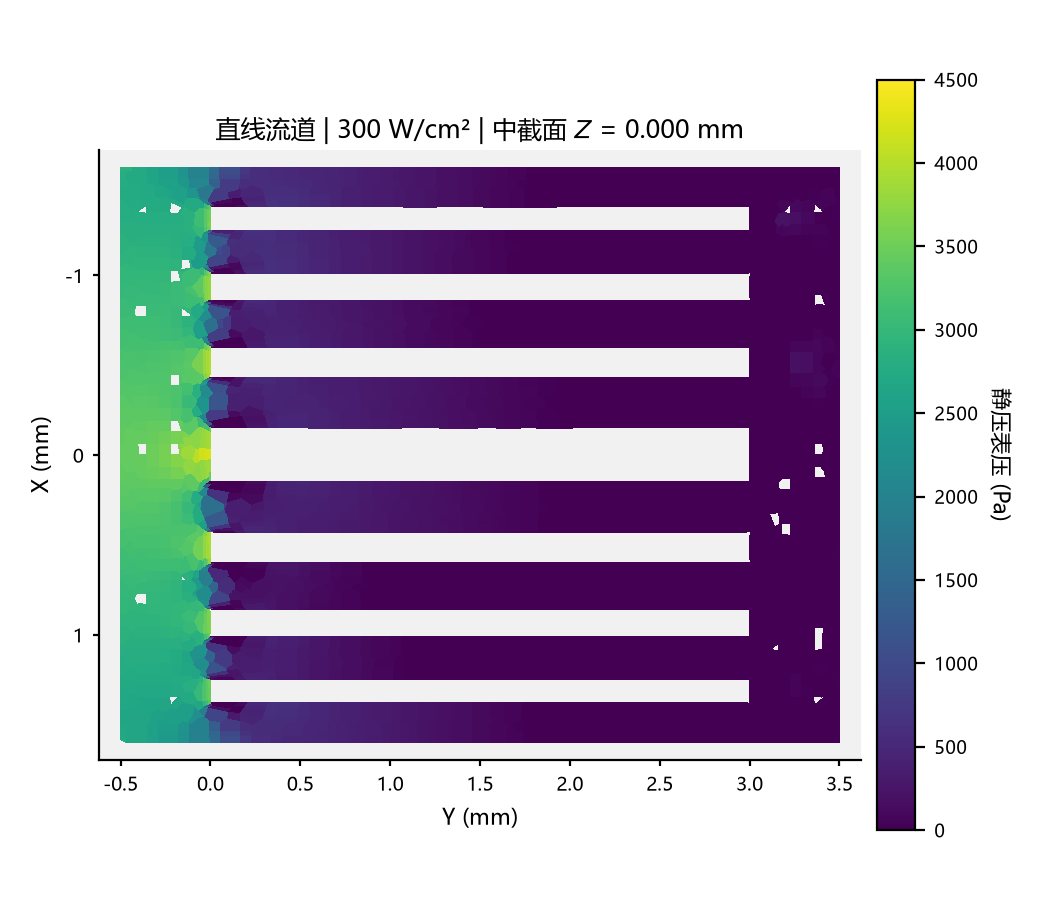
\includegraphics[width=\linewidth]{../../figs/15_zhixian_pressure.png}
		\caption{直线流道静压}
		\label{fig:zhixian-p}
	\end{subfigure}\hfill
	\begin{subfigure}{0.235\textwidth}
		\centering
		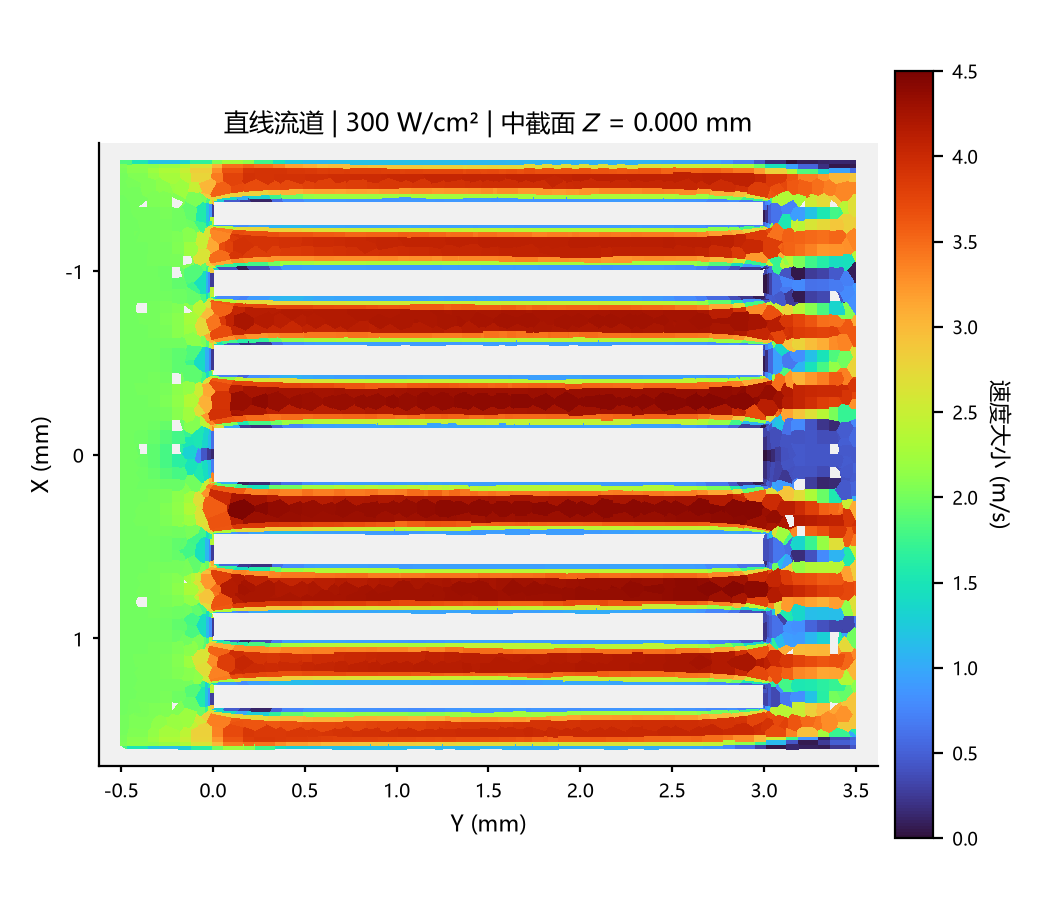
\includegraphics[width=\linewidth]{../../figs/16_zhixian_speed.png}
		\caption{直线流道速度大小}
		\label{fig:zhixian-v}
	\end{subfigure}\hfill
	\begin{subfigure}{0.235\textwidth}
		\centering
		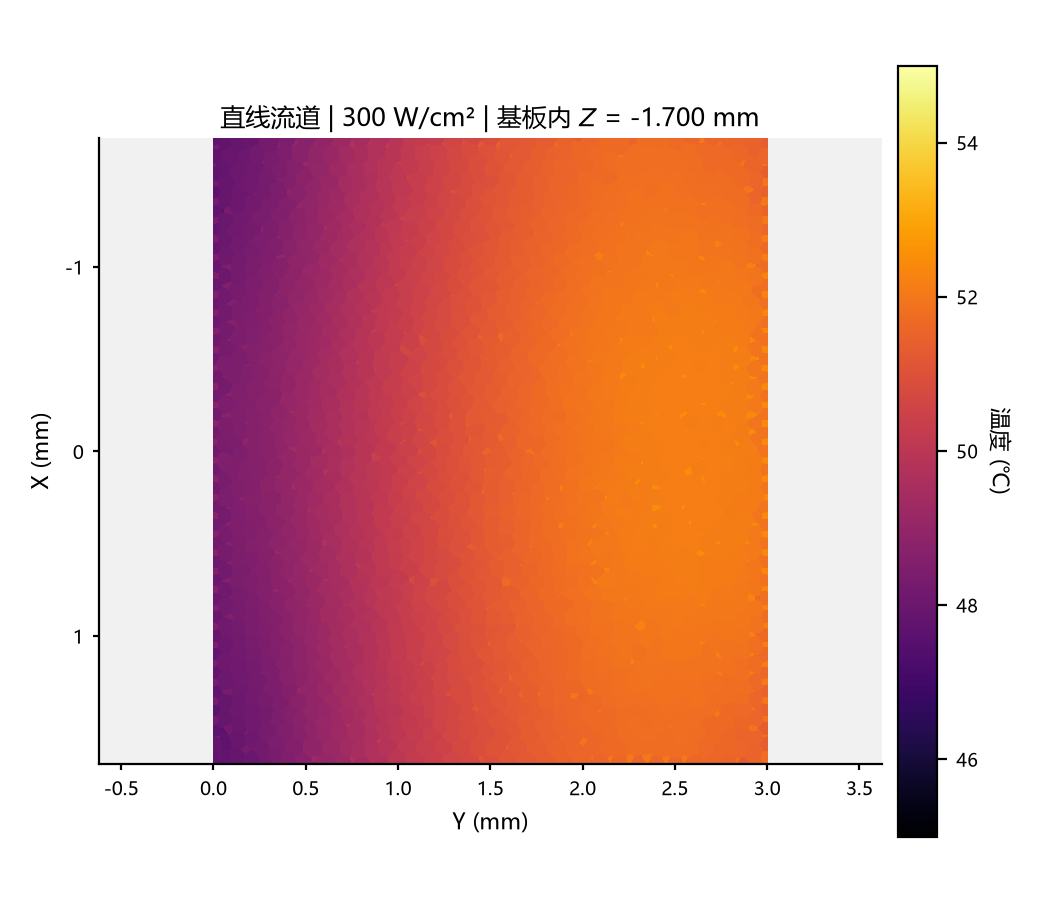
\includegraphics[width=\linewidth]{../../figs/17_zhixian_base_temperature.png}
		\caption{直线流道铜板温度}
		\label{fig:zhixian-cu}
	\end{subfigure}

	\vspace{4pt}

	\begin{subfigure}{0.235\textwidth}
		\centering
		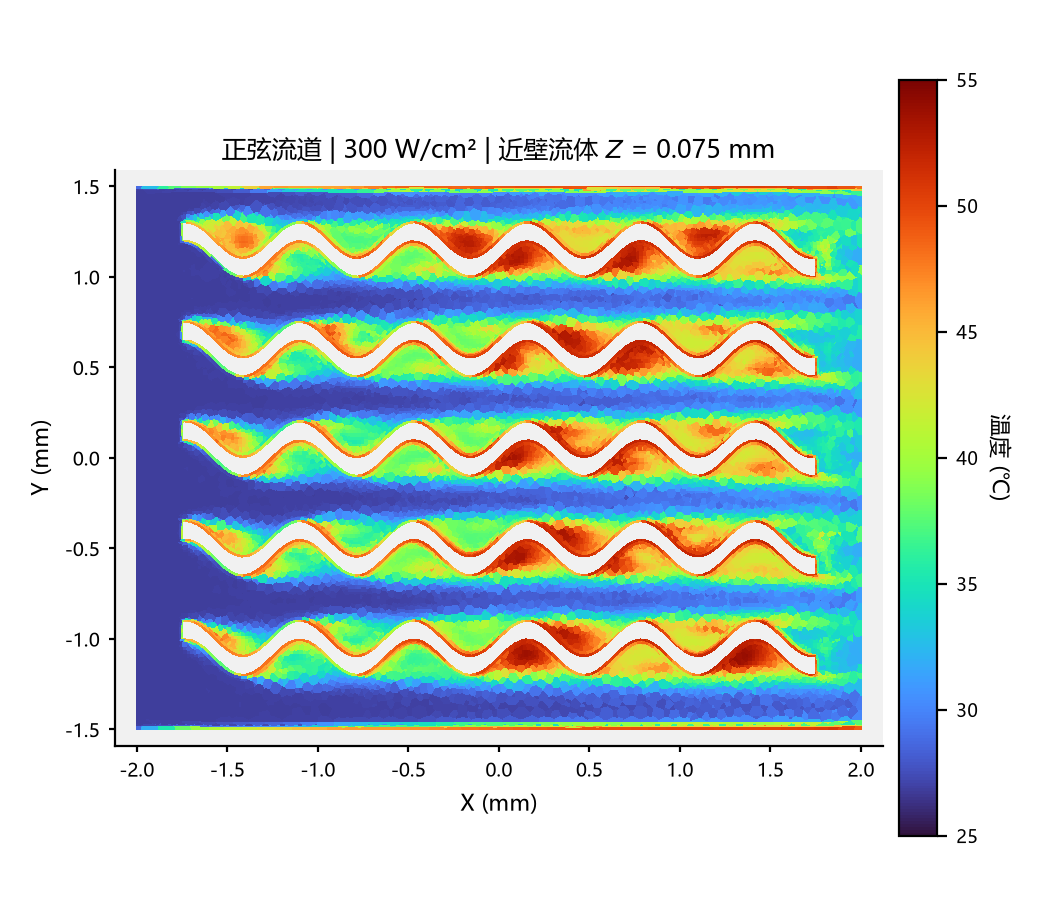
\includegraphics[width=\linewidth]{../../figs/18_sin_temperature.png}
		\caption{正弦流道温度}
		\label{fig:sin-t}
	\end{subfigure}\hfill
	\begin{subfigure}{0.235\textwidth}
		\centering
		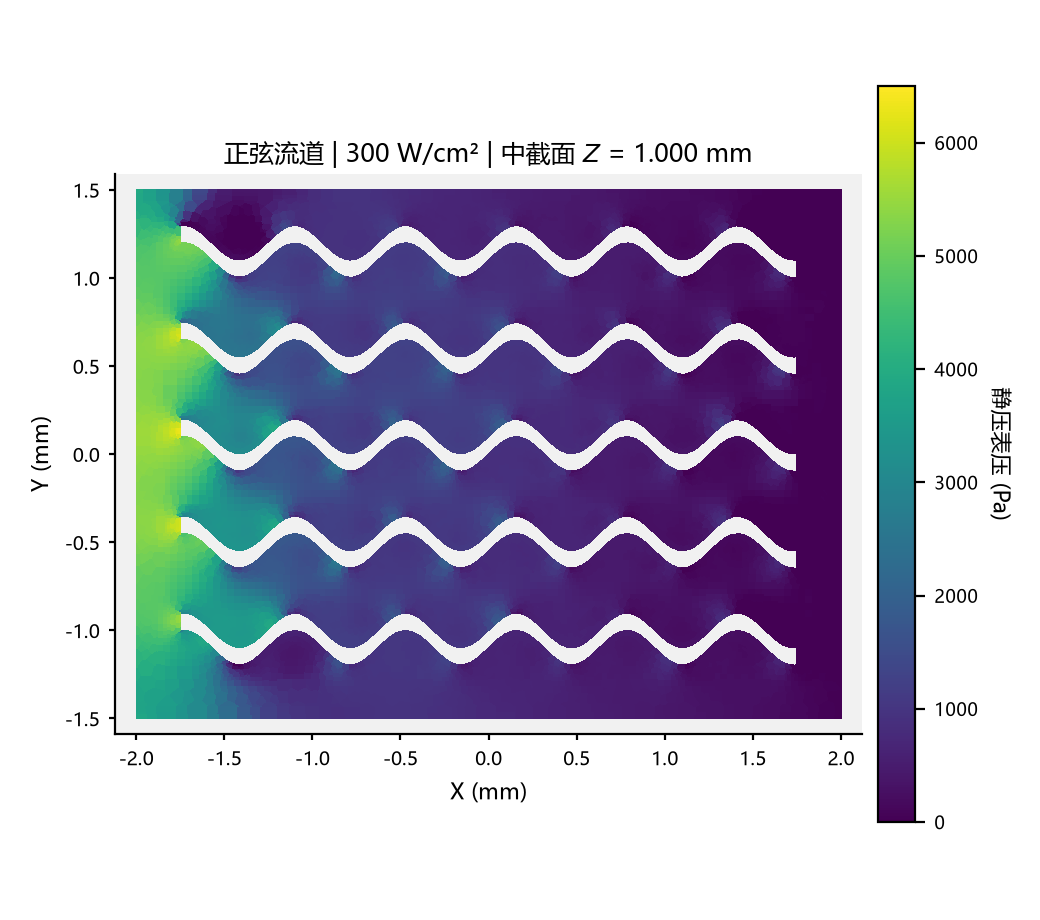
\includegraphics[width=\linewidth]{../../figs/19_sin_pressure.png}
		\caption{正弦流道静压}
		\label{fig:sin-p}
	\end{subfigure}\hfill
	\begin{subfigure}{0.235\textwidth}
		\centering
		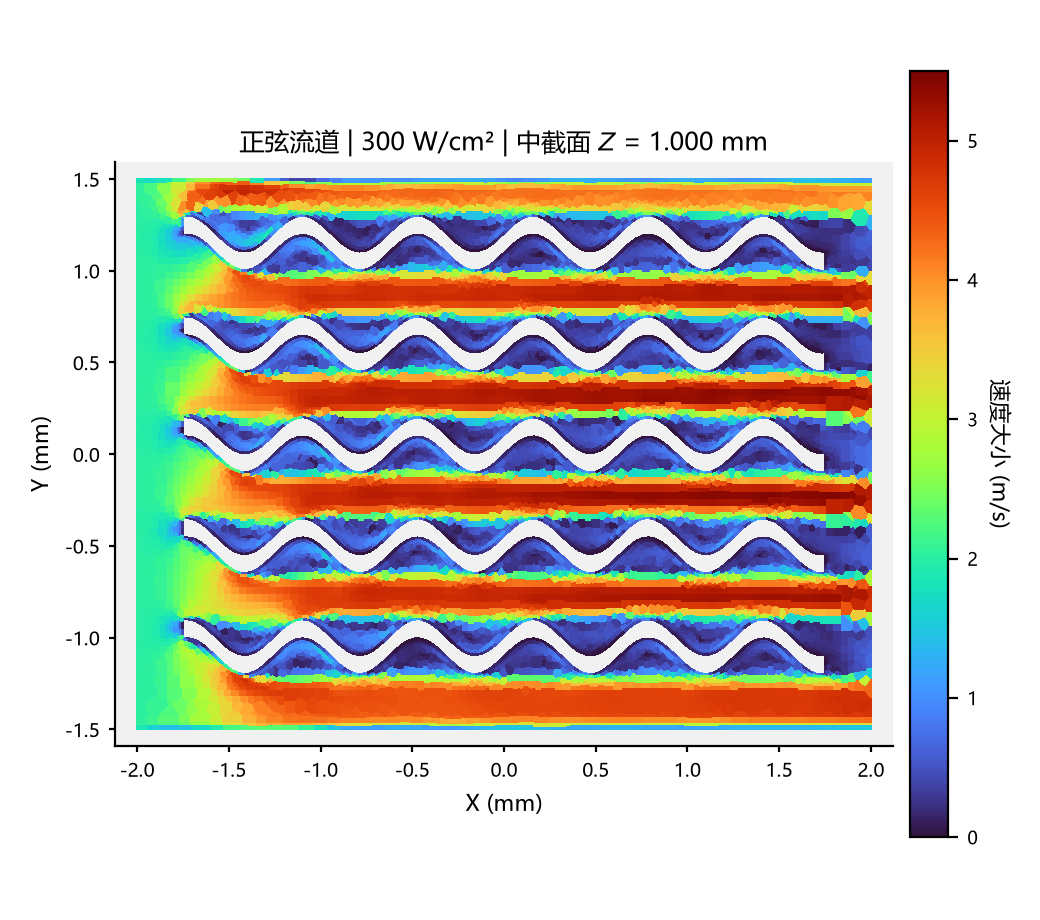
\includegraphics[width=\linewidth]{../../figs/20_sin_speed.png}
		\caption{正弦流道速度大小}
		\label{fig:sin-v}
	\end{subfigure}\hfill
	\begin{subfigure}{0.235\textwidth}
		\centering
		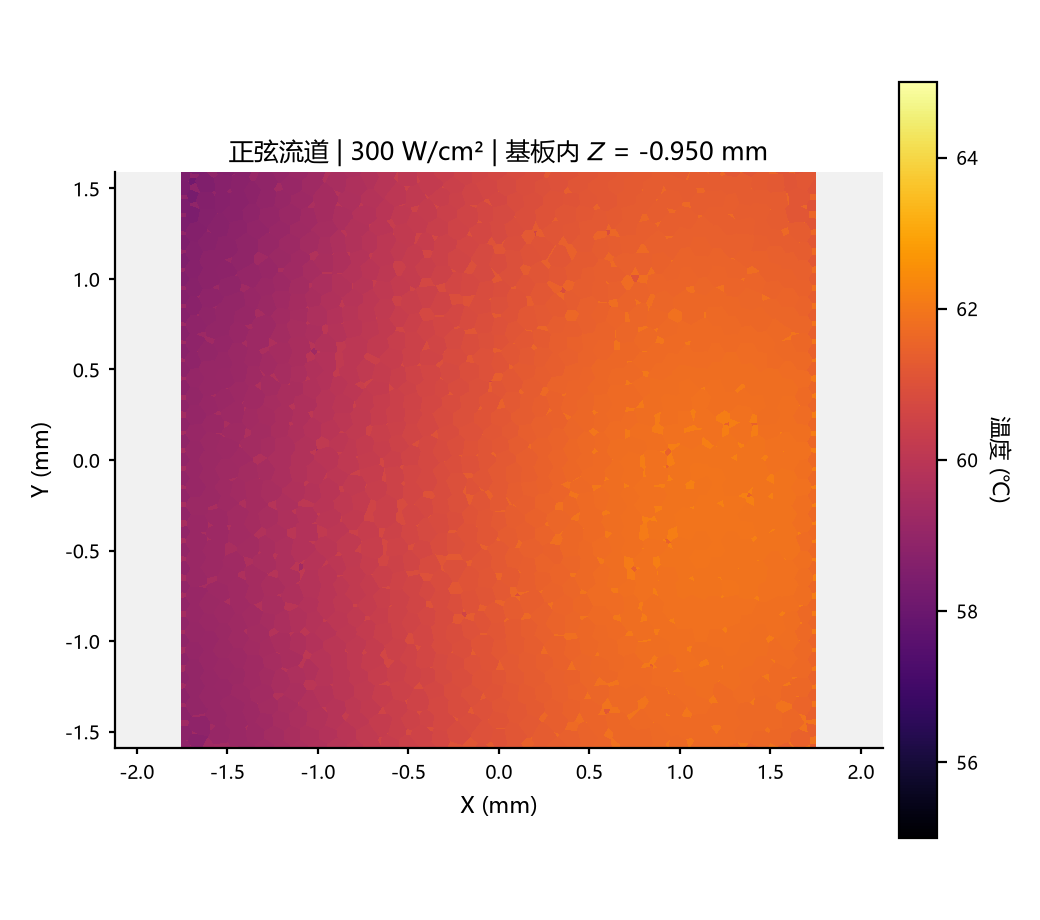
\includegraphics[width=\linewidth]{../../figs/21_sin_base_temperature.png}
		\caption{正弦流道铜板温度}
		\label{fig:sin-cu}
	\end{subfigure}

	\vspace{4pt}

	\begin{subfigure}{0.235\textwidth}
		\centering
		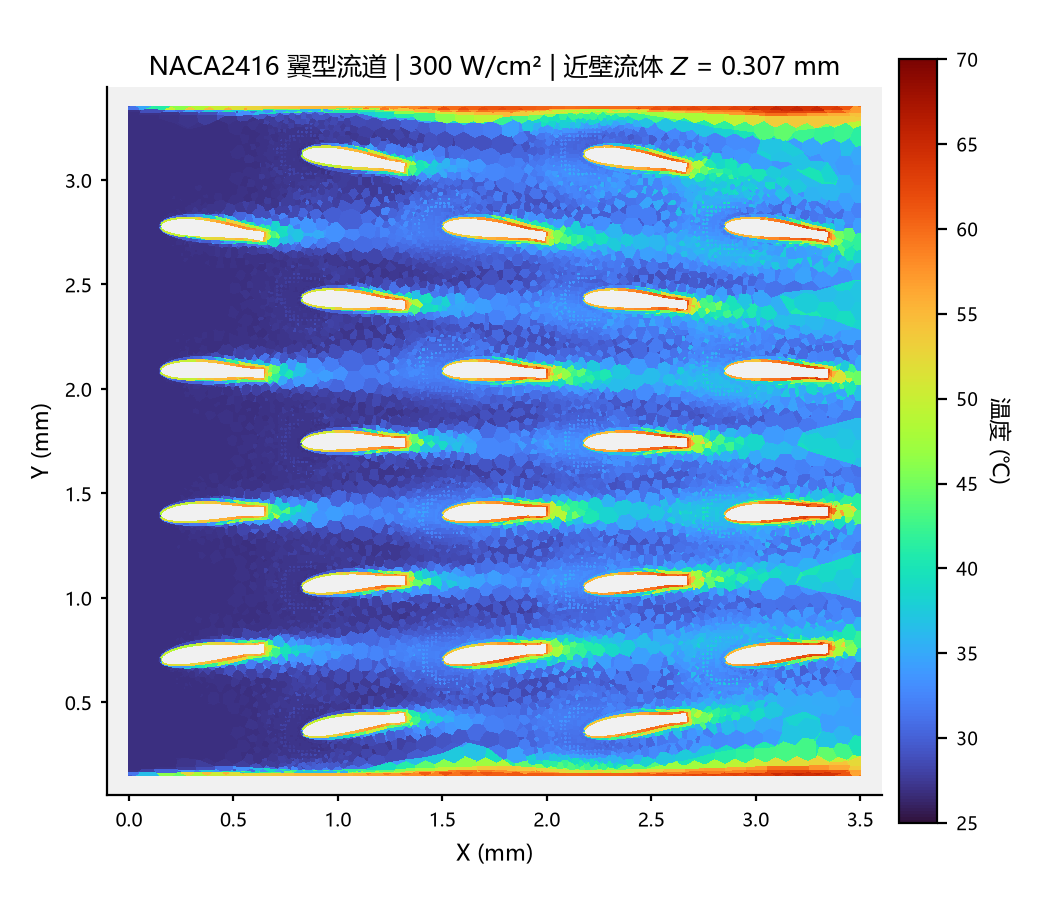
\includegraphics[width=\linewidth]{../../figs/22_naca_temperature.png}
		\caption{NACA2416 温度}
		\label{fig:naca-t}
	\end{subfigure}\hfill
	\begin{subfigure}{0.235\textwidth}
		\centering
		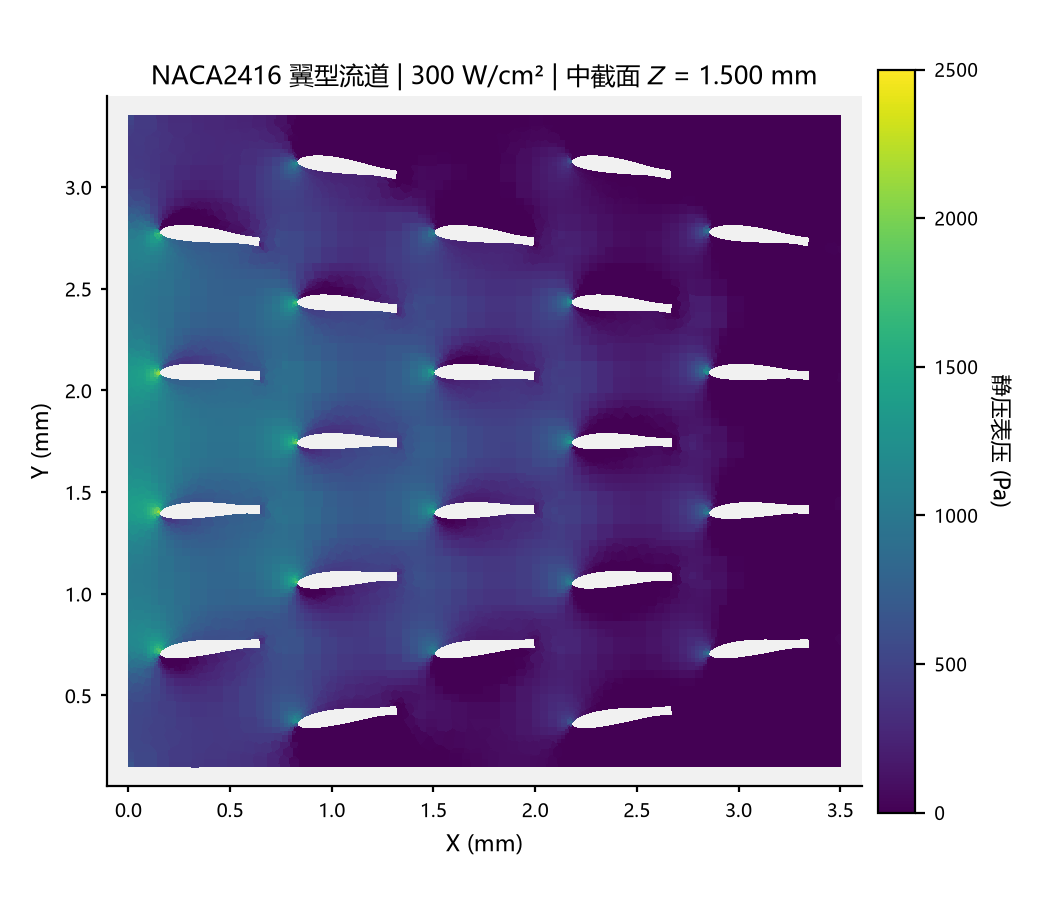
\includegraphics[width=\linewidth]{../../figs/23_naca_pressure.png}
		\caption{NACA2416 静压}
		\label{fig:naca-p}
	\end{subfigure}\hfill
	\begin{subfigure}{0.235\textwidth}
		\centering
		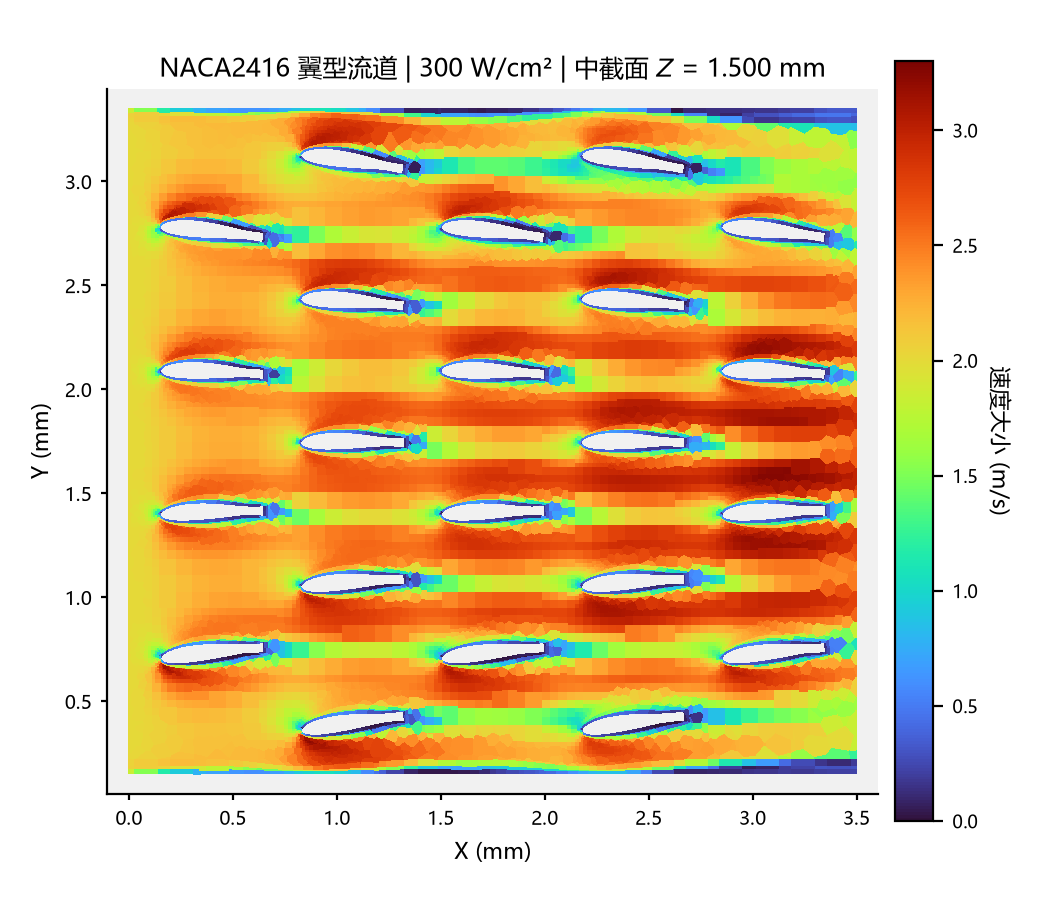
\includegraphics[width=\linewidth]{../../figs/24_naca_speed.png}
		\caption{NACA2416 速度大小}
		\label{fig:naca-v}
	\end{subfigure}\hfill
	\begin{subfigure}{0.235\textwidth}
		\centering
		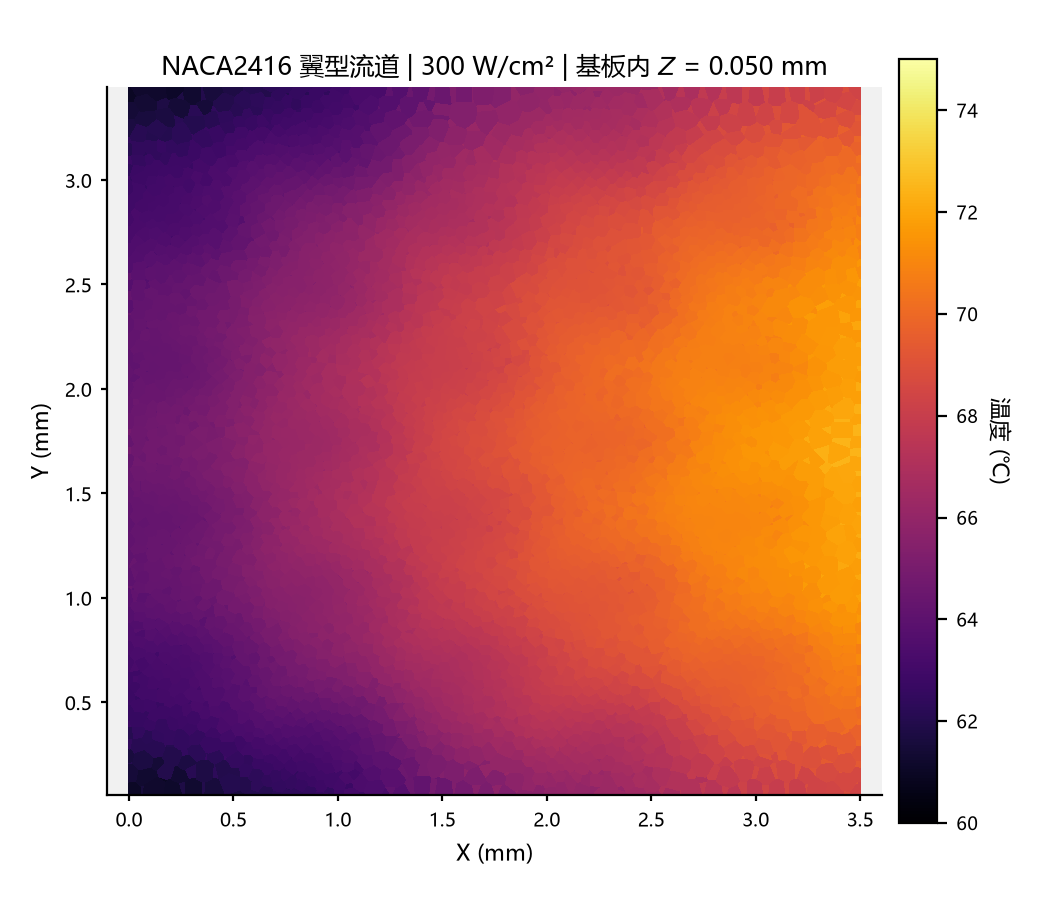
\includegraphics[width=\linewidth]{../../figs/25_naca_base_temperature.png}
		\caption{NACA2416 铜板温度}
		\label{fig:naca-cu}
	\end{subfigure}

	\vspace{4pt}

	\begin{subfigure}{0.235\textwidth}
		\centering
		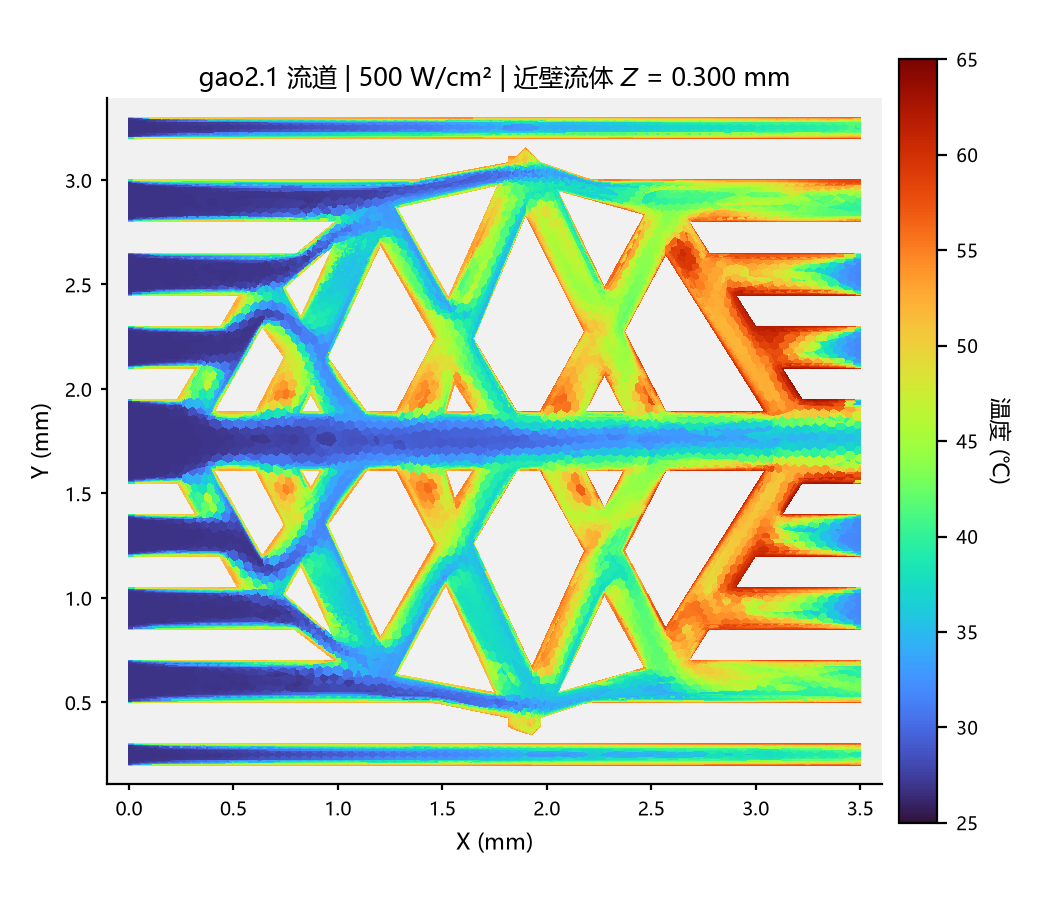
\includegraphics[width=\linewidth]{../../figs/26_gao_temperature.png}
		\caption{gao2.1 温度}
		\label{fig:gao-t}
	\end{subfigure}\hfill
	\begin{subfigure}{0.235\textwidth}
		\centering
		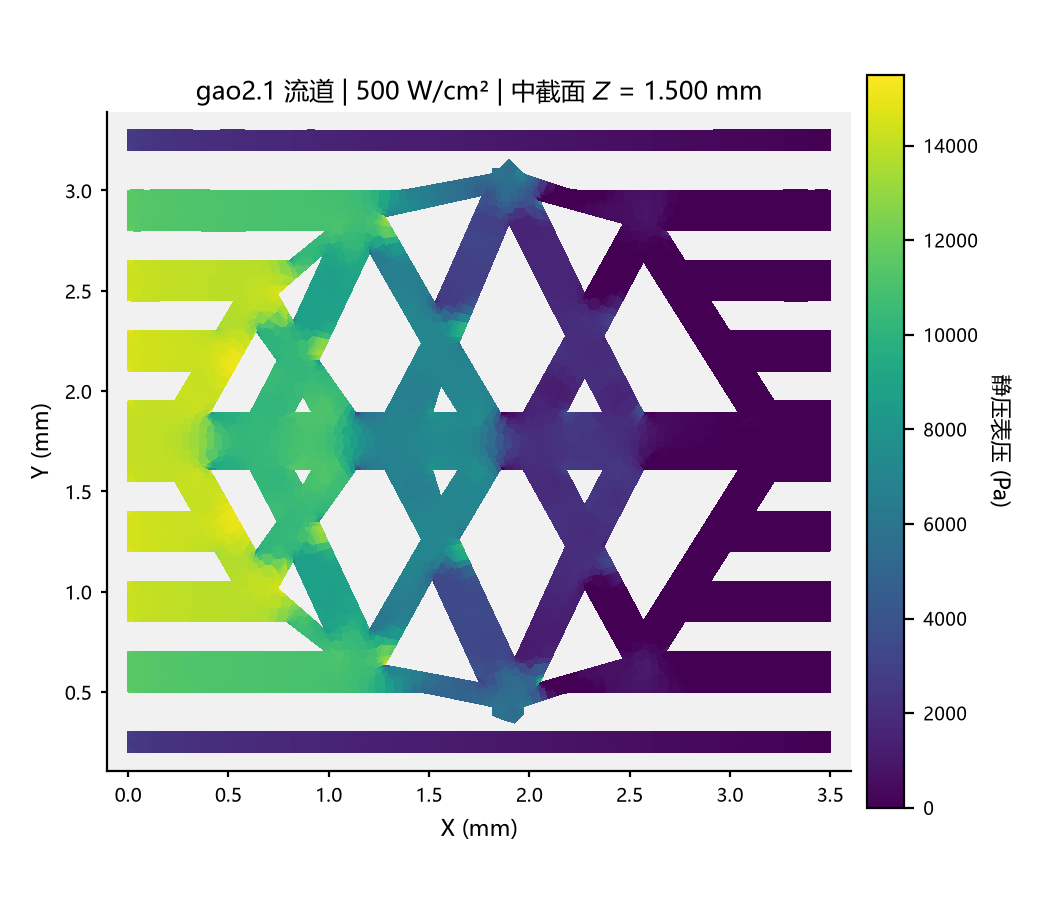
\includegraphics[width=\linewidth]{../../figs/27_gao_pressure.png}
		\caption{gao2.1 静压}
		\label{fig:gao-p}
	\end{subfigure}\hfill
	\begin{subfigure}{0.235\textwidth}
		\centering
		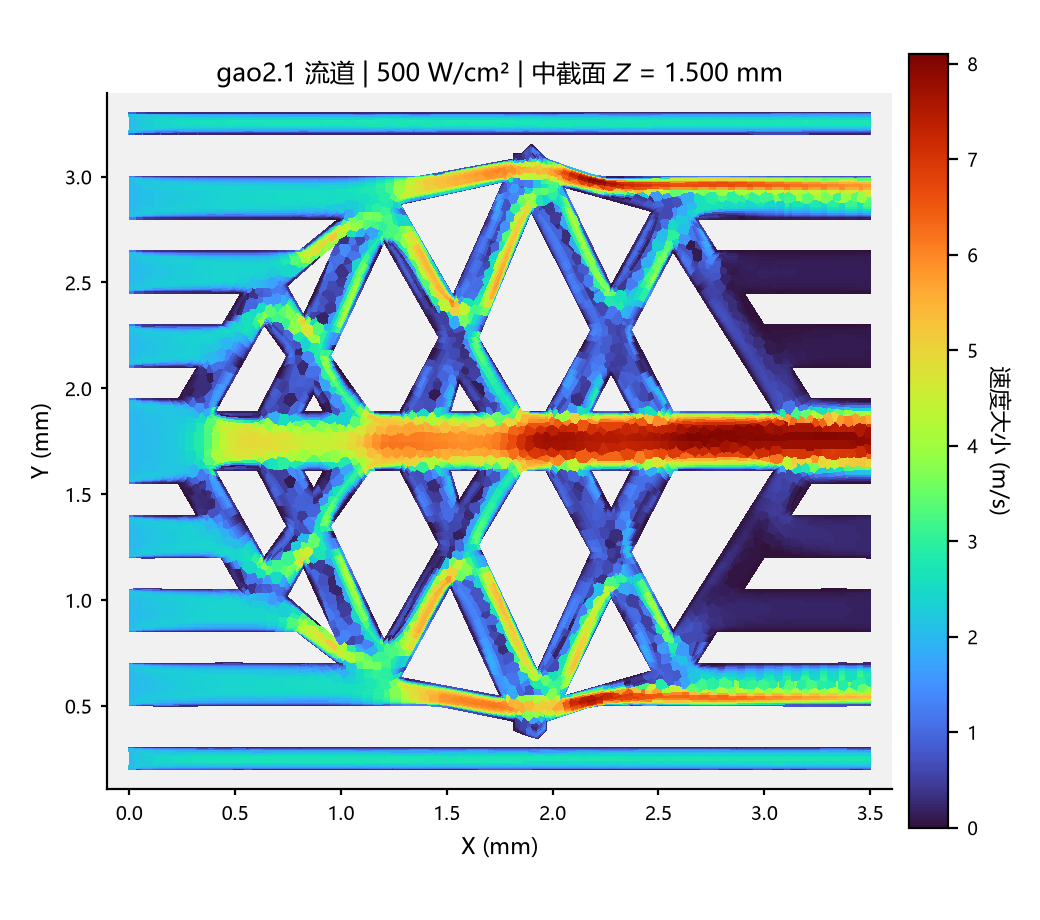
\includegraphics[width=\linewidth]{../../figs/28_gao_speed.png}
		\caption{gao2.1 速度大小}
		\label{fig:gao-v}
	\end{subfigure}\hfill
	\begin{subfigure}{0.235\textwidth}
		\centering
		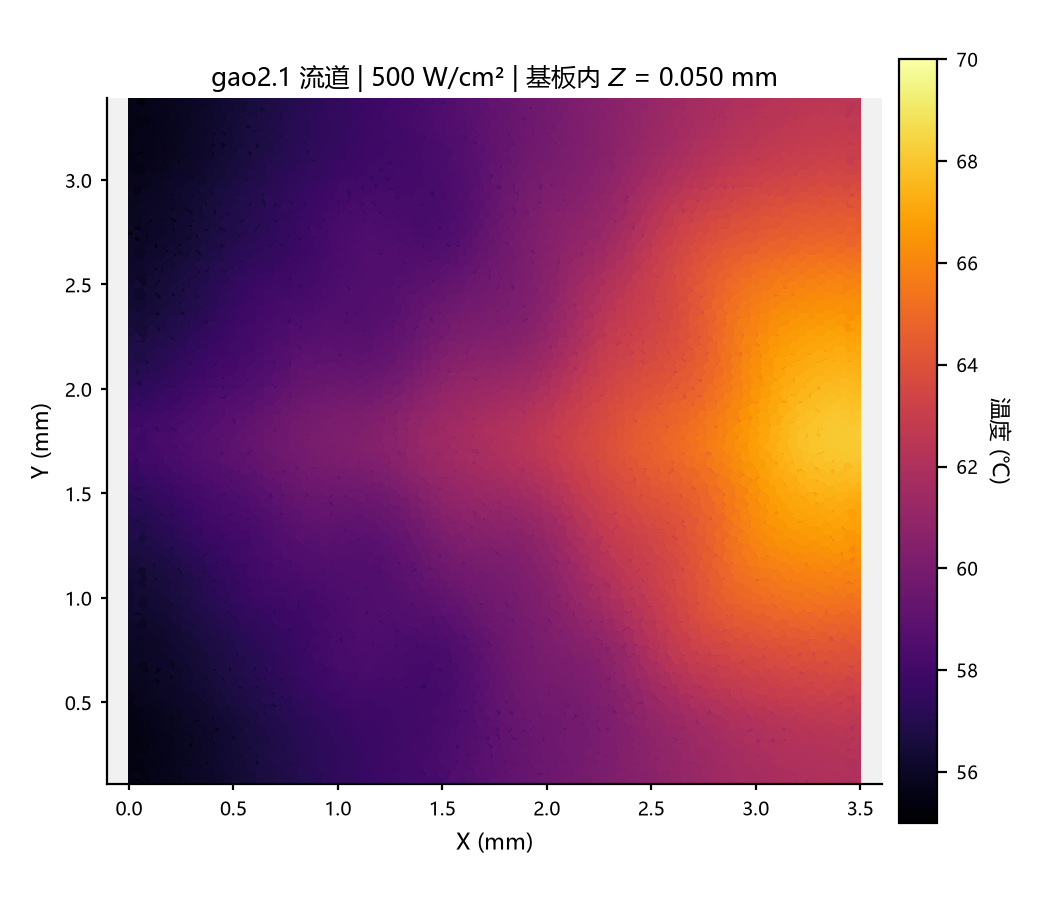
\includegraphics[width=\linewidth]{../../figs/29_gao_base_temperature.png}
		\caption{gao2.1 铜板温度}
		\label{fig:gao-cu}
	\end{subfigure}

\par\vspace{5pt}
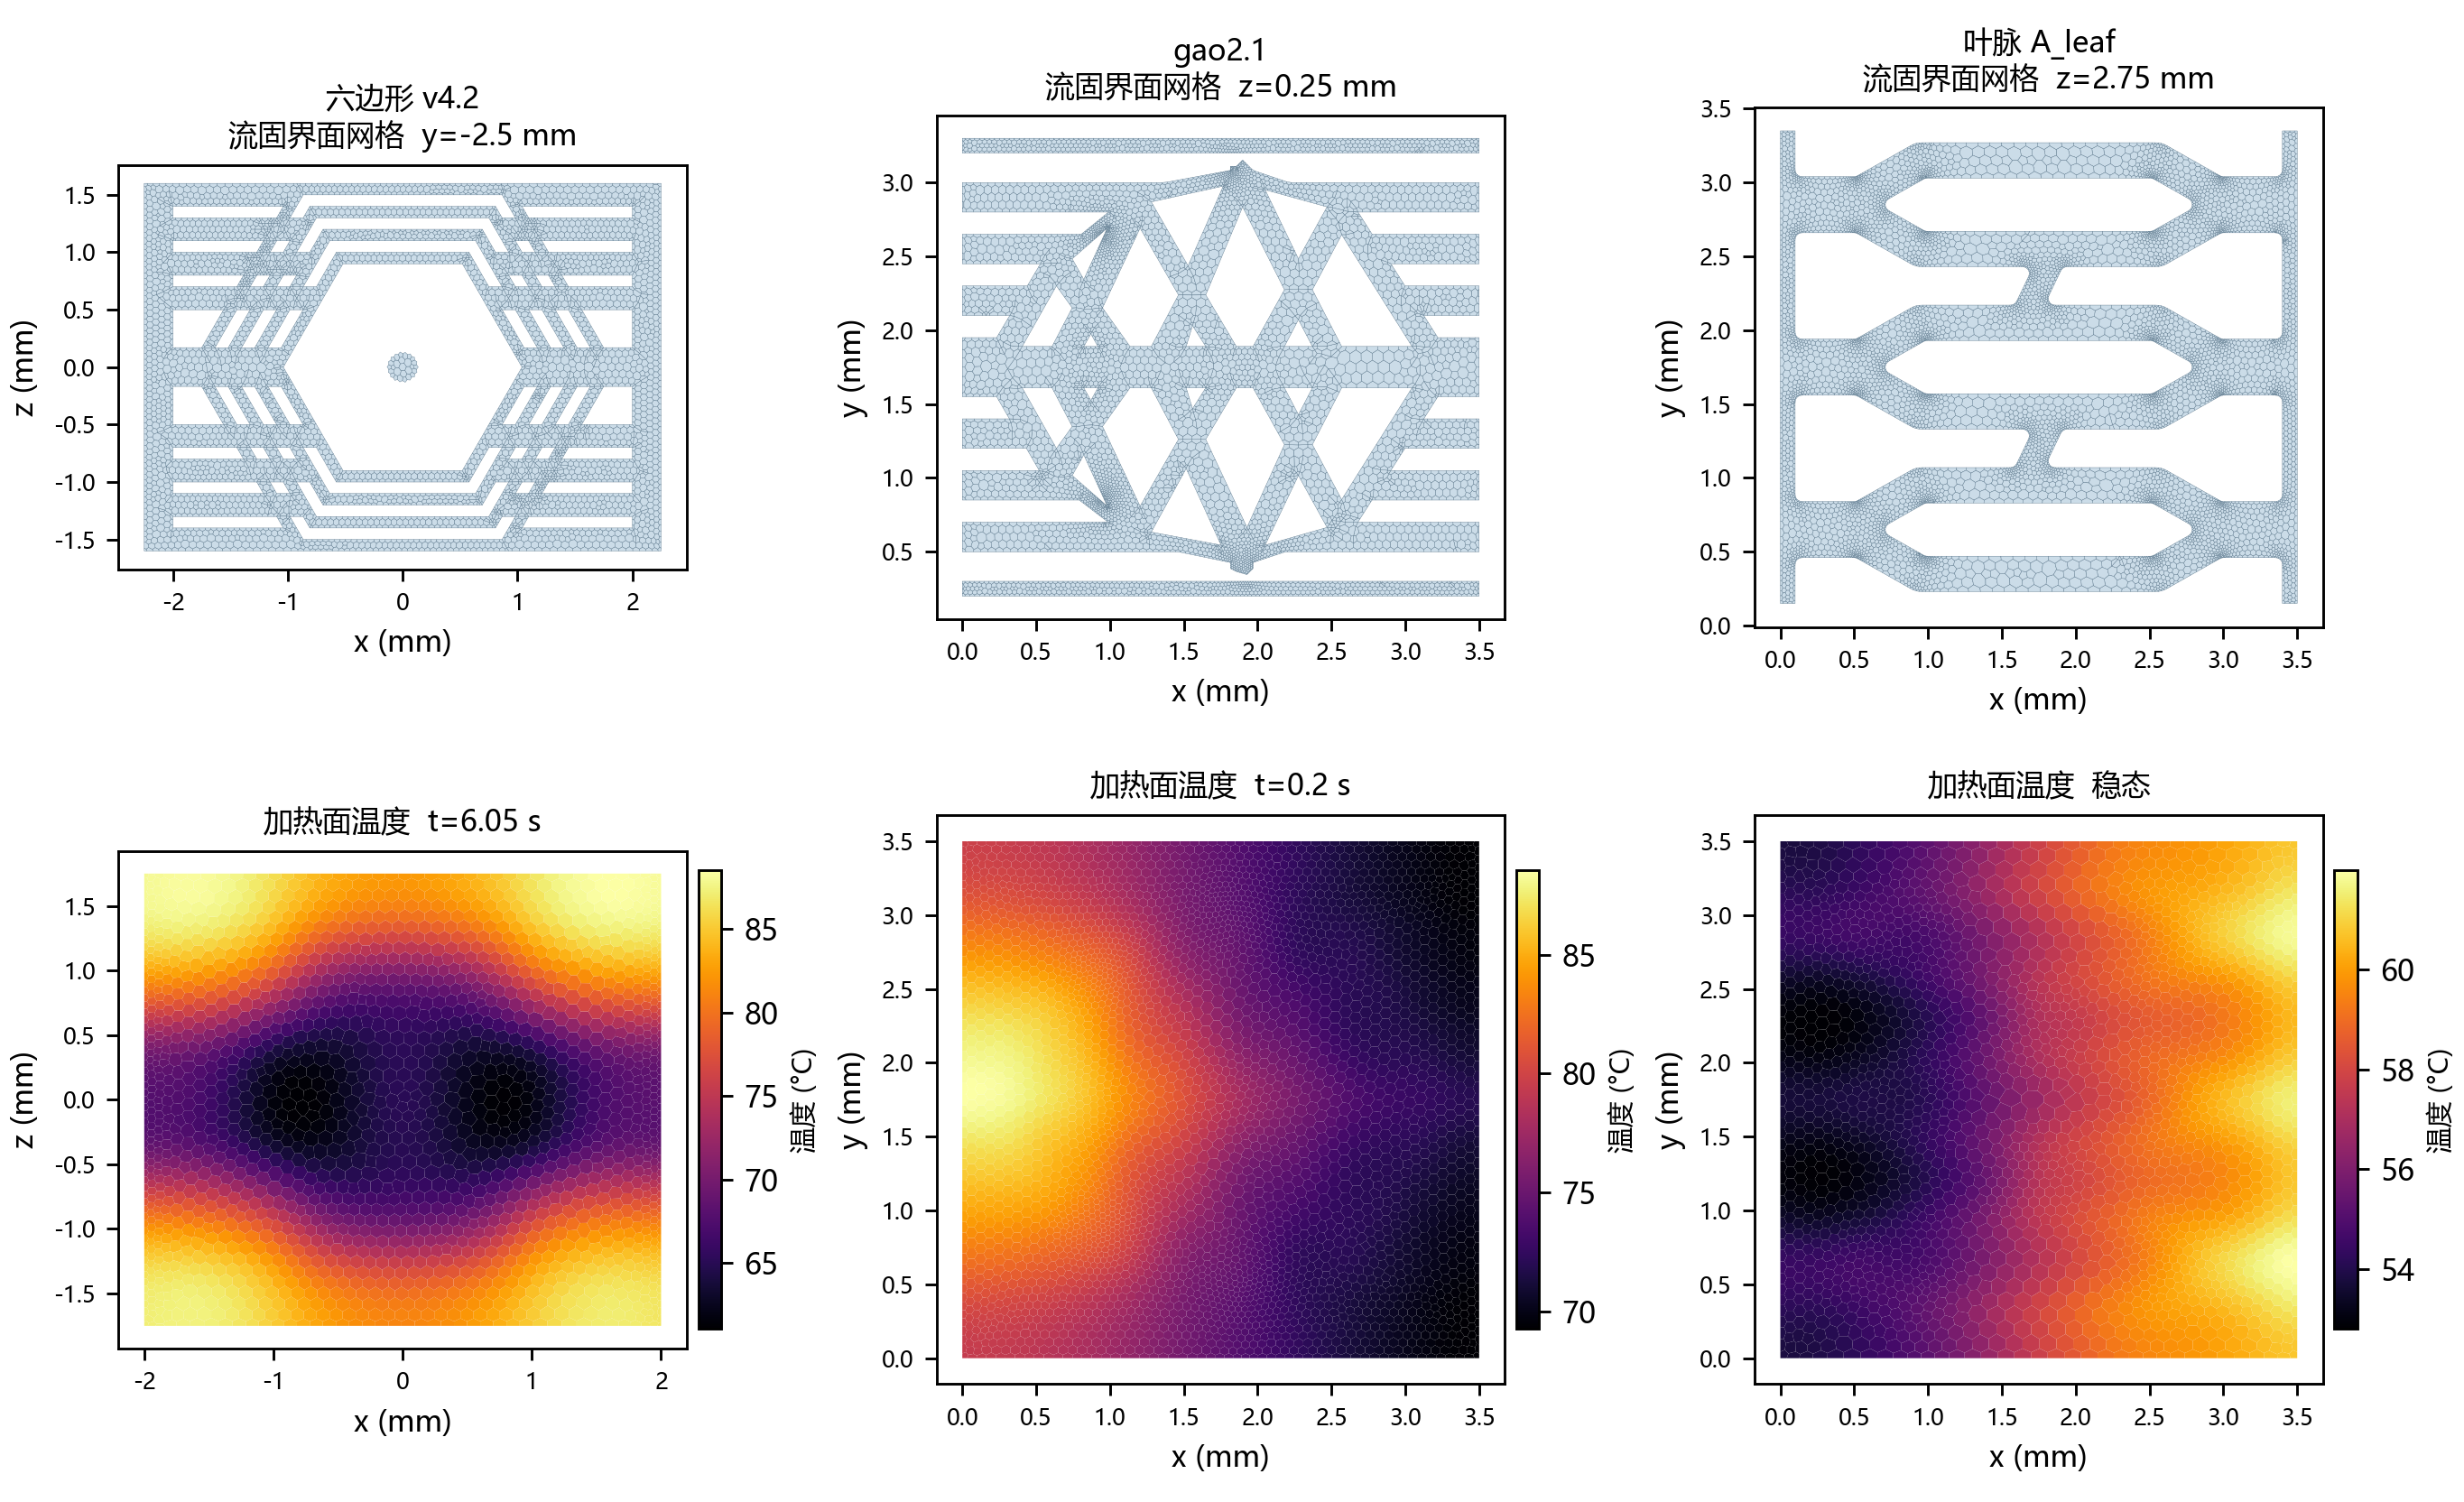
\includegraphics[width=0.84\linewidth]{../../figs/month2_other_models.png}
\end{minipage}%
}
\caption{流道与代表小模型的场分布及网格汇总。上部 (a)--(p) 按行依次为直线、正弦、NACA2416（均为 300 W/cm$^2$）及 gao2.1（500 W/cm$^2$），按列依次为近壁流体温度、静压、速度和铜板温度；下部三列依次为六边形 v4.2、gao2.1 与叶脉，上排为流固界面网格，下排为各自保存工况的加热面温度。各温度图色标独立，灰白区域为截面外或固体遮罩。}
\label{fig:contours}
\end{figure}
\clearpage
\setcounter{table}{5}
\begin{longtable}{@{}r p{0.30\textwidth} r r r r@{}}
\caption{流道与小模型的温度及水力性能汇总（按数据来源与工况分组）}
\label{tab:results}\\
\toprule
\rowcolor{ydzjlight} 热流密度 & 模型或分支 & 最高温度 & 平均温度 & 压差 & 水力功率 \\
/ (W/cm$^2$) & & / $^\circ$C & / $^\circ$C & / kPa & / W \\
\midrule
\endfirsthead
\caption[]{流道与小模型的温度及水力性能汇总（续）}\\
\toprule
\rowcolor{ydzjlight} 热流密度 & 模型或分支 & 最高温度 & 平均温度 & 压差 & 水力功率 \\
/ (W/cm$^2$) & & / $^\circ$C & / $^\circ$C & / kPa & / W \\
\midrule
\endhead
\midrule
\multicolumn{6}{r}{\small 接下页}\\
\endfoot
\bottomrule
\endlastfoot
300.00 & 直线 & 52.50 & 38.43 & 3.074 & 0.04919 \\
300.00 & 正弦 & 62.27 & 44.84 & 4.914 & 0.05897 \\
300.00 & NACA2416 & 72.48 & 45.99 & 0.979 & 0.01566 \\
500.00 & gao2.1 & 68.50 & 42.55 & 12.457 & 0.11211 \\
500.00 & NACA2416 & 99.60 & 56.82 & 0.926 & 0.01482 \\
350.00 & 六边形 v4 & 45.75 & 30.77 & 512.097 & 39.45329 \\
650.00 & 六边形 v4.2 & 88.26 & 49.50 & 78.587 & 1.17881 \\
350.00 & 0016 A06 基础 & 58.20 & 34.18 & 3.393 & 0.05428 \\
350.00 & 2416 A00 core & 71.03 & 40.07 & 2.456 & 0.03929 \\
350.00 & 2416 A00 BOI & 71.01 & 39.25 & 2.512 & 0.04019 \\
350.00 & 0016 A06 拟合物性 & 59.61 & 34.62 & 4.290 & 0.06864 \\
350.00 & 0016 A06 REFPROP & 59.54 & 34.59 & 4.290 & 0.06864 \\
350.00 & 2416 v3 & 72.83 & 38.74 & 2.348 & 0.03757 \\
600.00 & gao2.1 & 88.41 & 53.57 & 13.969 & 0.12572 \\
126.82 & 2420 v4 原始 & 43.08 & 31.40 & 1.377 & 0.01653 \\
126.82 & 2420 回流 300 K & 44.23 & 31.83 & 1.651 & 0.01988 \\
126.82 & 2420 IAPWS dt0.005 & 44.32 & 31.87 & 1.652 & 0.01989 \\
126.82 & 2420 IAPWS dt0.01 & 44.32 & 31.87 & 1.652 & 0.01989 \\
450.00 & 0016 v2 & 85.34 & 43.21 & 2.248 & 0.03596 \\
450.00 & 1416 v2 & 85.31 & 43.46 & 2.255 & 0.03609 \\
450.00 & 3416 v2 & 85.11 & 43.12 & 2.366 & 0.03785 \\
600.00 & 叶脉 A\_leaf & 61.81 & 37.92 & 47.668 & 0.76269 \\
\end{longtable}
\clearpage
\setcounter{table}{6}
\begin{table}[H]\centering\small
\caption{全部小模型的流量与保存条件}\label{tab:other-conditions}
\begin{tabularx}{\textwidth}{@{}Y r r r@{}}
\toprule
\rowcolor{ydzjlight} 分支 & 流量 / (mL/s) & 保存时刻 / s & 时间步 / s \\
\midrule
六边形 v4 & 77.043 & 15 & 0.5 \\
六边形 v4.2 & 15.000 & 6.05 & 0.01 \\
0016 A06 基础 & 16.000 & 0.1 & 0.01 \\
2416 A00 core & 16.000 & 0.15 & 0.01 \\
2416 A00 BOI & 16.000 & 0.2 & 0.01 \\
0016 A06 拟合物性 & 16.000 & 0.2 & 0.001 \\
0016 A06 REFPROP & 16.000 & 0.137 & 0.001 \\
2416 v3 & 16.000 & 0.2 & 0.001 \\
gao2.1 & 9.000 & 0.2 & 0.01 \\
2420 v4 原始 & 12.000 & 1 & 0.01 \\
2420 回流 300 K & 12.041 & 1 & 0.01 \\
2420 IAPWS dt0.005 & 12.041 & 1 & 0.005 \\
2420 IAPWS dt0.01 & 12.041 & 1 & 0.01 \\
0016 v2 & 16.000 & 0.1 & 0.0002 \\
1416 v2 & 16.000 & 0.1 & 0.0002 \\
3416 v2 & 16.000 & 0.1 & 0.0002 \\
叶脉 A\_leaf & 16.000 & 稳态 & --- \\
\bottomrule
\end{tabularx}
\end{table}
\clearpage
\setcounter{table}{7}
\begin{table}[H]
\centering
\caption{不同翼型构型流热耦合仿真关键结果（基准工况）}
\label{tab:airfoil-overview}
\begin{tabularx}{\textwidth}{@{}l c c c c@{}}
\toprule
\rowcolor{ydzjlight} 构型 & 最高温度 / K & 底板平均温度 / K & $h$ / (W/(m$^2$·K)) & PEC \\
\midrule
NACA0015 & 357.9 & 356.1 & 756.6 & 1.00 \\
NACA0021 & 355.7 & 354.0 & 765.3 & 1.10 \\
NACA0024 & 354.9 & 353.2 & 798.5 & 1.19 \\
NACA4424 & 354.4 & 352.7 & 789.8 & 1.21 \\
NACA6424 & 358.1 & 356.3 & 750.5 & 1.00 \\
NACA6624 & 357.9 & 356.1 & 750.2 & 1.01 \\
\bottomrule
\end{tabularx}
\end{table}
\clearpage
\setcounter{table}{8}
\begin{table}[H]\centering
\caption{后续工作及所需产出}\label{tab:plan}
\begin{tabularx}{\textwidth}{@{}Y Y Y@{}}
\toprule
\rowcolor{ydzjlight} 工作 & 状态 \\
\midrule
翼型参数分组研究 & 明确变量、固定条件与缺失数据 \\
正式修改 UDF 与网格检验 & 适用范围、校验和敏感性记录  \\
PID 纯数学模拟 & 保存时序、统计窗口及实现检查  \\
\bottomrule\end{tabularx}\end{table}
\clearpage
\begin{thebibliography}{9}

\bibitem{smallmodels} 小模型保存结果与性能汇总. 项目仿真资料, 2026. 见配套数据文件 small\_model\_results.csv 及 model\_sources.json；数值由 Case／Data 提取，图像由实际面元及表面温度生成。
\bibitem{airfoil} 微通道液冷场景下的翼型参数. 项目资料, 2026.
\bibitem{control} 控制理论与 PID 算法相关资料. 项目资料, 2026.

% ---------- 控制理论学习书籍（张昊洋补充）----------
\bibitem{hushousong} 胡寿松. 自动控制原理[M]. 8 版. 北京: 科学出版社, 2023.
\bibitem{astrom} {\AA}STR{\"O}M K J, H{\"A}GGLUND T. PID Controllers: Theory, Design, and Tuning[M]. 2nd ed. Research Triangle Park: Instrument Society of America, 1995.
\bibitem{franklin} FRANKLIN G F, POWELL J D, EMAMI-NAEINI A. Feedback Control of Dynamic Systems[M]. 8th ed. London: Pearson, 2019.
\bibitem{ogata} OGATA K. Modern Control Engineering[M]. 5th ed. London: Pearson, 2010.
\bibitem{brunton} BRUNTON S L, KUTZ J N. Data-Driven Science and Engineering: Machine Learning, Dynamical Systems, and Control[M]. 2nd ed. Cambridge: Cambridge University Press, 2022.
\bibitem{wu} 吴睿康. 电子器件主动液冷散热的建模及实验研究[D]. 杭州: 浙江大学, 2020.
\bibitem{ji} 季俊杰. 微通道冷却芯片及其热点的动态特性研究[D]. 杭州: 浙江大学, 2021.
\bibitem{laguna} LAGUNA G, VILARRUBI M, IBANEZ M, et al. Numerical parametric study of a hotspot-targeted microfluidic cooling array for microelectronics[J]. Applied Thermal Engineering, 2018, 144: 71-80.
\end{thebibliography}
\end{document}
